\documentclass[tikz,border=10pt]{standalone}
\usepackage{fontspec}
\setmainfont{Latin Modern Roman}
\usetikzlibrary{arrows.meta}
\begin{document}
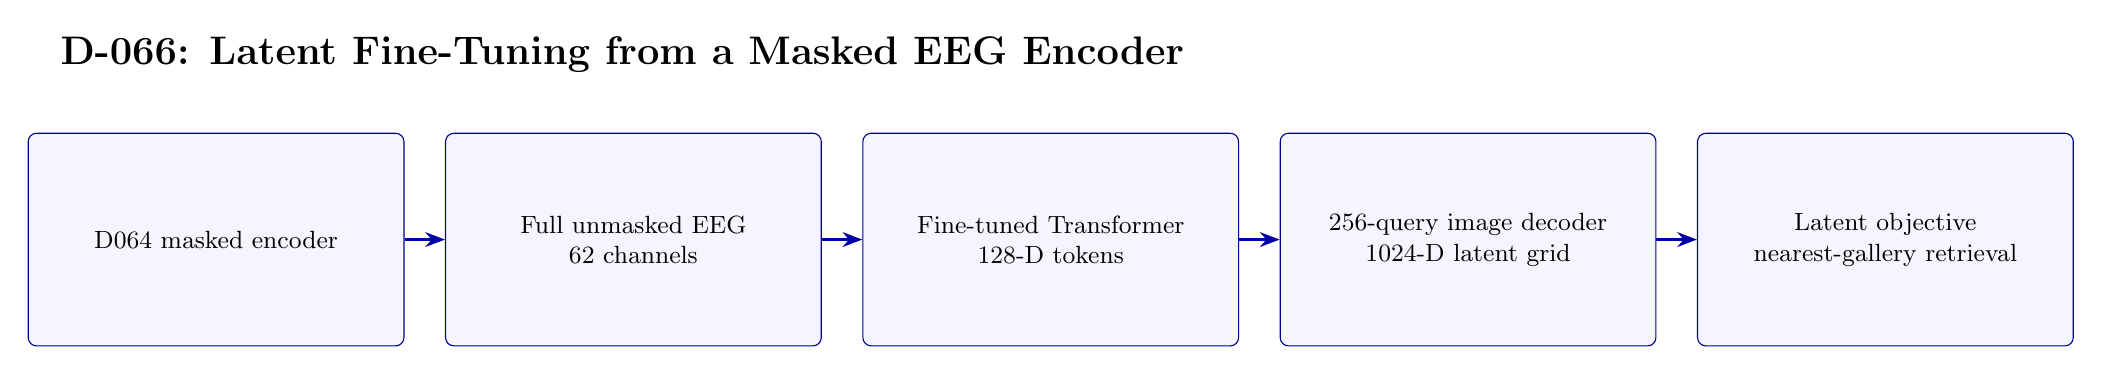
\begin{tikzpicture}[block/.style={draw=blue!55!black,fill=blue!4,rounded corners=3pt,align=center,text width=4.35cm,minimum height=2.7cm,inner sep=6pt,font=\small},arrow/.style={-{Stealth[length=2.5mm]},line width=1pt,draw=blue!65!black}]
\node[font=\Large\bfseries,anchor=south west] at (-2.1,2.0) {D-066: Latent Fine-Tuning from a Masked EEG Encoder};
\node[block] (n0) at (0.0,0) {D064 masked encoder};
\node[block] (n1) at (5.3,0) {Full unmasked EEG\\62 channels};
\node[block] (n2) at (10.6,0) {Fine-tuned Transformer\\128-D tokens};
\node[block] (n3) at (15.899999999999999,0) {256-query image decoder\\1024-D latent grid};
\node[block] (n4) at (21.2,0) {Latent objective\\nearest-gallery retrieval};
\draw[arrow] (n0) -- (n1);
\draw[arrow] (n1) -- (n2);
\draw[arrow] (n2) -- (n3);
\draw[arrow] (n3) -- (n4);
\end{tikzpicture}
\end{document}
